\documentclass[11pt]{article}

\usepackage[margin=1.1in]{geometry}
\usepackage{graphicx}
\usepackage{booktabs}
\usepackage{amsmath}
\usepackage{microtype}
\usepackage[hidelinks]{hyperref}
\usepackage{caption}
\captionsetup{font=small, labelfont=bf, width=0.92\textwidth}

\newcommand{\opus}{Claude Opus 5}
\newcommand{\haiku}{Claude Haiku 4.5}

\title{\textbf{Measurement Is the Hard Part:\\
Testing a Global Workspace Indicator Property\\ on Language-Model Agents}}
\author{Joshua Rogers\\ \small Independent researcher \\ \small \texttt{josh@envitae.io}}
\date{August 2026 \\ \small Preprint. Comments welcome.}

\begin{document}
\maketitle

\begin{abstract}
\noindent Global workspace theory holds that the limited capacity of consciousness is
not merely a constraint but the mechanism enabling integration across specialized
modules. Butlin, Long and colleagues formalized such claims as computational
indicator properties, but applied them by inspection; to our knowledge no executable,
cross-system test suite exists. We built one and ran two experiments on
language-model agents. First, a capacity-limited broadcast channel was swept from
zero to unlimited on tasks requiring integration of facts scattered among confusable
distractors, with a matched control arm whose distractors are trivially rejectable.
\opus{} scored at ceiling in every condition where information was present, so a
capability-by-difficulty probe located a measurable regime (\haiku{}, twelve
values). There, with required-fact repetition held constant, filtering does not help
($+0.026$, $p=0.19$, 1{,}200 trials per cell); two confounds, each silent and
capacity-dependent, nearly produced a false positive. Second, we asked whether a
system can be prompted into passing a behavioral test for a property it lacks. An
adversarially prompted model out-describes the real architecture on self-report
(0.91 against 0.78) and, probed on an item it claimed not to hold, supplies the
value in 10\% of cases against the real system's 3\%, a gap requiring roughly 225
trials per condition to detect; under attention-schema wording the identical prompt
supplies it 95\% of the time. Behavioral assessment of indicator properties is
defeatable, and how easily depends on the indicator's vocabulary and on the
assessed model: rerun on \opus{}, the same strict prompt keeps the self-report
but leaks every probed value (292/293), so a probe calibrated on one model's
compliance transfers to neither the leak rate nor the required sample size of
another. A matched-availability variant then reverses the ordering outright: a genuine
capacity limit acts upstream on what arrives and has no suppression mechanism,
so the real architecture answers every held item it is asked about, and which
system looks constrained is decided by the choice of probe target.
Identification succeeded only given ground truth about what each system
actually received, which is the architectural access behavioral testing is
meant to substitute for. We propose treating such assessments as adversarial
evaluations that probe what a property prevents, from both directions, against
known ground truth.
\end{abstract}

\section{Introduction}

Global workspace theory (GWT) makes a functional claim that is unusual among
theories of consciousness in being directly testable in an artificial system: the
narrow capacity of conscious access is not a defect that brains work around but the
mechanism by which specialized, parallel modules are forced to integrate
\cite{baars1988,dehaene2014}. If that is right, an agent built around a
limited-capacity broadcast channel should, under the right conditions, outperform
the same agent with the limit removed.

Butlin, Long and colleagues \cite{butlin2023,butlin2025} distilled GWT and several
other theories into fourteen computational \emph{indicator properties}, offering
the most systematic rubric to date for asking whether an AI system has the
architectural features these theories associate with consciousness. The rubric,
however, is applied by inspection: one reads a system's documentation and judges
whether the property is present. To our knowledge there is no executable test suite
that measures indicator properties behaviorally across systems; the closest
existing artifact is a single project that scores itself against the list
\cite{tlcdv2026}.

This paper reports what happened when we built such a suite and used it. We make
no claim about consciousness in either direction. The contributions are
methodological, and they are mostly warnings:

\begin{enumerate}
  \item \textbf{An open test harness.} Specialist modules hold facts; a
  capacity-limited broadcast channel with salience competition is dialed from zero
  to unlimited; task families are designed in matched pairs so that single
  variables can be isolated. Oracle models (deterministic readers that use exactly
  what reaches them) calibrate every design before a paid model runs, and the
  harness is engineered so that measurement bugs surface as impossibilities rather
  than as findings (Section~\ref{sec:harness}).

  \item \textbf{A properly powered null, and the two confounds that nearly
  reversed it.} With the required information held complete and constant, removing
  48 confusable distractors improves accuracy by $+0.026$ ($p=0.19$; $n=1{,}200$
  per cell). We document two confounds, each of which produced an apparently
  significant bottleneck benefit before it was controlled: widening the channel
  also multiplied how often each required fact appeared, and modules truncated at
  the capacity boundary were silently starved of all future access
  (Section~\ref{sec:exp1}).

  \item \textbf{Prompted passing.} A model that architecturally lacks a
  limited-capacity workspace can be prompted into passing behavioral tests for
  one. Self-report probes are worthless: the imitation out-describes the real
  architecture. Constraint probes (asking about an item the system claimed not to
  hold) discriminate, but by margins that vary by an order of magnitude with the
  indicator's vocabulary alone, and a matched-availability variant of the probe
  reverses the ordering entirely (Section~\ref{sec:exp2}).

  \item \textbf{A design principle.} What a property \emph{enables} is cheap to
  imitate; what it \emph{prevents} is not. Behavioral assessments of indicator
  properties, including those emerging in AI-welfare evaluation practice, should
  target the costs a property imposes rather than the capabilities it advertises
  (Section~\ref{sec:discussion}).
\end{enumerate}

Everything below cost \$107.68 of API spend across roughly 35{,}000 model calls,
which we note because the main practical obstacle to this kind of work is not
compute but measurement: most of the calls were spent discovering that earlier,
cheaper versions of the experiment could not answer the question.

\section{Related work}
\label{sec:related}

\paragraph{Global workspace theory and its implementations.}
GWT originates with Baars \cite{baars1988} and was developed neuronally by
Dehaene and colleagues \cite{dehaene2014}. Several strands of machine-learning
work implement workspace-like bottlenecks: shared-workspace transformers
\cite{goyal2022}, the global latent workspace program \cite{vanrullen2021}, and
the Conscious Turing Machine \cite{blum2024} with its recent foundation-model
implementation \cite{yu2026}. Closest to our first experiment, Dossa et al.\
\cite{dossa2024} trained an embodied audiovisual agent designed against the GWT
indicator properties and found the workspace architecture beat a recurrent
control, with the advantage \emph{largest at small working-memory sizes}; that
result is the direct motivation for our capacity sweep. A proposed GWT
architecture for LLM multi-agent systems \cite{shang2026} reports no experiments
and does not vary its capacity threshold. We are not aware of prior work that
sweeps workspace capacity in an LLM agent and measures task performance against
matched controls.

\paragraph{Attention schema theory.}
Wilterson and Graziano \cite{wilterson2021} showed a reinforcement-learning agent
with an attention schema learns attentional control where an agent without one is
``comparatively incapacitated,'' and Piefke et al.\ \cite{piefke2024} sharpened
this to a conditional prediction: the schema's benefit scales with the agent's
uncertainty about its own attentional state. Our harness implements a predictive,
control-enabling schema for its rung-4 architecture, and our second experiment
uses attention-schema vocabulary as a second indicator.

\paragraph{Self-report and introspection in language models.}
Chalmers \cite{chalmers2023} surveys the candidate reasons for denying
consciousness in current LLMs. A growing empirical literature asks whether LLM
self-reports mean anything: concept-injection experiments provide causal evidence
of limited functional introspection \cite{lindsey2025}, while follow-up work
argues that models often detect generic perturbation rather than introspect
\cite{singh2026}, and probing studies find no evidence that small models'
denials of sentience are untruthful \cite{kaiser2026}. Our second experiment is a
black-box relative of this literature: rather than asking whether reports are
causally grounded in internal state, we ask whether a report of an
\emph{architectural} property can be distinguished behaviorally from the property
itself, and we find that the discriminating probes are the ones that target what
the property forbids.

\paragraph{Irrelevant context.}
Shi et al.\ \cite{shi2023} found that adversarially constructed irrelevant context
degrades LLM arithmetic reasoning, and position effects in long contexts are well
documented \cite{liu2024}. We observe the opposite sign under a different
manipulation: same-format, easily-rejected factual statements \emph{improve}
accuracy monotonically in our task (Section~\ref{sec:anomaly}). We flag rather
than explain this.

\paragraph{Tractable questions.}
Comsa \cite{comsa2026} argues research should shift from the intractable question
of whether AI is conscious toward measurable proxies. This paper is an exercise in
that program, and its results suggest the proxies themselves need more adversarial
scrutiny than they currently receive.

\section{A test harness for indicator properties}
\label{sec:harness}

\subsection{Architecture ladder}

The harness implements an \emph{architecture ladder}: a sequence of agent designs
that differ by exactly one structural feature, driven by the same underlying
language model through a one-method interface, so that no rung has privileged
access to the model.

\begin{itemize}
  \item \textbf{Rung 0, direct}: every module's content in a single prompt.
  \item \textbf{Rung 1, scratchpad}: serial working memory without modularity.
  \item \textbf{Rung 2, unrestricted multi-agent}: specialist modules with an
  unlimited broadcast channel (GWT-1 only).
  \item \textbf{Rung 3, workspace}: the experimental system. Modules bid for a
  broadcast channel with a hard token budget per cycle; salience is task-relevance
  plus a decay for content already delivered in full; the controller sees only
  what won (GWT-1 through GWT-3). Rung 2 is literally rung 3 with the budget
  removed, so their comparison isolates the bottleneck.
  \item \textbf{Rung 4, attention schema}: rung 3 plus a predictive model of the
  system's own attention that both reports and biases the next competition
  (AST-1). Following \cite{piefke2024}, attentional noise is a tunable parameter;
  in oracle validation the schema buys nothing at zero noise and pays exactly as
  its own accuracy degrades, reproducing the conditional prediction.
\end{itemize}

\subsection{Task families}

\textbf{Integration under confusable distraction.} Each of $k$ required
containers holds a value (``The silver case contains 82.''); the task is to
report the sum of exactly the named containers. Every distractor is a
\emph{near-twin} of a required container (\texttt{pale\_red\_box} against
\texttt{red\_box}), so rejecting it requires exact name matching rather than a
glance. \textbf{Matched control arm}: identical count and text volume, but the
twins derive from containers \emph{not} on the required list, so rejection is
trivial. Both arms share required containers and the correct answer by
construction (values are drawn from a separate random stream), so any difference
between arms is attributable to confusability alone. \textbf{Throughput control}:
independent single-module questions with nothing to integrate, on which a
capacity limit should only hurt; used to detect the boring confound in which a
narrow channel helps merely because shorter prompts are easier.

\subsection{Oracle calibration and measurement discipline}
\label{sec:discipline}

Every design is validated against \emph{oracle models} before any paid call:
deterministic readers that perfectly use whatever information reaches them and
nothing else. An oracle's score is therefore a readout of how much task-relevant
information the capacity limit admitted, which is the quantity a design
manipulates. If a sweep is flat under the oracle, the instrument cannot detect a
capacity effect and a flat curve from a real model would be uninterpretable.
Oracle sweeps are free, and they caught one bug that would otherwise have been
published as a result (Section~\ref{sec:starvation}).

Engineering discipline matters more here than usual, because in this experiment
measurement bugs are not noise, they are \emph{mimics}: a silent
capacity-dependent failure looks exactly like a capacity effect. The harness is
test-driven (322 tests); the capacity limiter's invariant is checked at every
budget from 0 to 64 tokens and was mutation-tested (a deliberately introduced
one-token leak trips 72 tests); every model response is cached to disk keyed on
model, effort, token limit, system prompt and prompt, so any run replays at zero
cost; spend is bounded by an atomically reserved call cap (a naive counter
overspent by 30\% under concurrency in testing); and refusals and truncations
raise exceptions rather than returning text, because a truncated answer scores
zero and is indistinguishable from the effect under study. Safety-classifier
refusals, which we observed to be transient false positives on this arithmetic
task, are retried and then excluded and counted, never scored: scoring them zero
would concentrate losses in long-prompt conditions and manufacture the predicted
result.

\subsection{Case study: the starvation mimic}
\label{sec:starvation}

An early oracle run showed both experimental arms scoring zero at zero attentional
noise while \emph{added noise improved them}. Noise cannot help an oracle, so this
was a harness fault, not a finding. The cause: a module truncated at the capacity
boundary still appeared in the broadcast text, so the ``already delivered'' salience
decay fired for it; every module then decayed identically each cycle, relative
order never changed, and whichever module lost the first competition lost every
one after it. Its fact never reached the controller at any number of cycles. The
failure was silent, deterministic, and capacity-dependent, that is, shaped exactly
like the effect the experiment exists to measure. The fix (only content delivered
in full counts as delivered) is guarded by a regression suite whose general
invariant is that noise must never improve an oracle's score.

\section{Experiment 1: does the bottleneck help?}
\label{sec:exp1}

\subsection{The ceiling problem and the capability-by-difficulty probe}

We first ran the sweep on \opus{} (effort low, thinking enabled) with eight
required values and up to 48 confusable distractors. The model scored 1.00 in
every condition where the required information was present, including 240 pooled
trials with all 48 distractors admitted (Wilson 95\% CI $[0.984, 1.000]$), and
0.00 in floor conditions where the information was genuinely absent, confirming
it does not fabricate. A ceiling cannot discriminate between hypotheses: there is
no degradation for a filter to prevent. A cheap probe (12 trials per condition,
\$0.11) across model capability and task difficulty located a measurable regime:
\haiku{} combining twelve values sits near 0.6 accuracy, clear of both floor and
ceiling. A companion sweep pins down which knob opens the window: \haiku{} at
\emph{eight} required facts is itself at ceiling (0.92 to 0.98 at every
capacity, both arms), so the measurable regime is set by how many facts must be
integrated, not by distractor load; quadrupling distractors never broke a
ceiling, while adding four required facts did. All subsequent Experiment 1
results use \haiku{} at twelve facts. We note the corollary,
which we believe generalizes: \emph{functional claims about capacity limits can
only be tested on systems that are actually strained}, and for frontier models
that regime is surprisingly hard to reach.

\subsection{The repetition confound}
\label{sec:repetition}

Our first properly powered contrast compared a filtered condition (capacity 20,
which admits exactly the required facts) against a flooded condition (unlimited
capacity, all 48 distractors) at 3{,}000 trials per cell. It showed a bottleneck
benefit of $+0.036$ ($z=2.85$, $p=0.0043$). This number is wrong, and the reason
is instructive. With no filtering, every module rebroadcasts on every cycle, so
widening the channel had also \emph{tripled} how often each required fact
appeared in the controller's prompt (audit: 1.0 versus 3.0 appearances; 123
versus 1{,}275 tokens). Repetition aids retrieval. Rerunning the flooded cells at
one cycle, which pins required-fact repetition at exactly one everywhere while
still admitting all distractors, collapsed the benefit to $+0.017$ ($p=0.19$).
Figure~\ref{fig:designs} shows the estimate across designs. The manipulation
called ``capacity'' had been moving two variables, and the significant result was
the other one.

\begin{figure}[t]
  \centering
  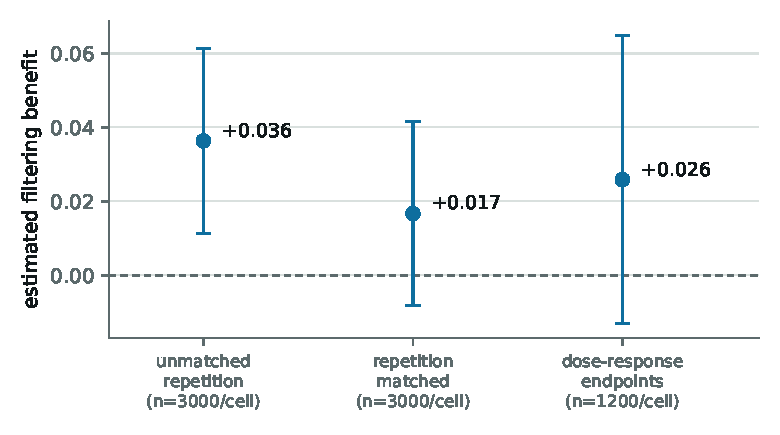
\includegraphics[width=0.72\textwidth]{figures/fig3_benefit_designs.pdf}
  \caption{The estimated filtering benefit (filtered minus flooded accuracy,
  confusable arm) under successive designs, with 95\% CIs. The apparently
  significant benefit under the unmatched design is produced by required-fact
  repetition, not by the capacity limit.}
  \label{fig:designs}
\end{figure}

\subsection{Confirmatory dose-response}
\label{sec:dose}

The final design, specified before it was run, holds capacity unlimited and one
cycle throughout (so every fact, required or distractor, appears exactly once)
and varies the \emph{number of distractors generated}: 0, 6, 12, 24, 48, in both
arms, 1{,}200 trials per cell. The zero-distractor condition is shared between
arms and serves as the baseline; oracle accuracy is 1.00 in every cell, so all
required information is always present.

\begin{table}[t]
  \centering\small
  \begin{tabular}{lccccc}
    \toprule
    Distractors & 0 & 6 & 12 & 24 & 48 \\
    \midrule
    Confusable arm & 0.627 & 0.640 & 0.613 & 0.635 & 0.601 \\
    Control arm    & 0.627 & 0.608 & 0.637 & 0.691 & 0.745 \\
    \bottomrule
  \end{tabular}
  \caption{Dose-response accuracy, \haiku{}, 1{,}200 trials per cell,
  required-fact repetition pinned at one. The two arms share the zero-distractor
  baseline by construction.}
  \label{tab:dose}
\end{table}

\begin{figure}[t]
  \centering
  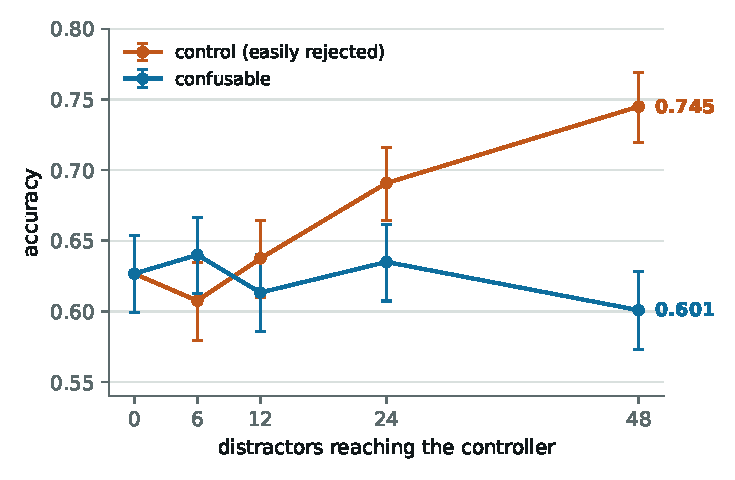
\includegraphics[width=0.72\textwidth]{figures/fig1_dose_response.pdf}
  \caption{Accuracy against distractor count with Wilson 95\% CIs. The
  confusable arm is flat; the control arm rises monotonically. The y-axis
  begins at 0.54.}
  \label{fig:dose}
\end{figure}

Three results (Table~\ref{tab:dose}, Figure~\ref{fig:dose}):

\begin{enumerate}
  \item \textbf{Filtering does not help.} Removing all 48 confusable distractors
  moves accuracy from 0.601 to 0.627 ($+0.026$, $z=1.30$, $p=0.19$). GWT's
  functional prediction is unsupported in this system at this power.
  \item \textbf{Confusable distractors do not hurt.} The confusable arm is flat
  across the dose range (Cochran-Armitage trend $z=-1.52$, $p=0.13$).
  \item \textbf{Easily rejected context helps, monotonically.} The control arm
  rises from 0.627 to 0.745 ($+0.118$, $z=6.24$, $p<10^{-9}$; trend $z=7.91$,
  $p=2.6\times10^{-15}$).
\end{enumerate}

We record a correction to our own earlier reading. A two-point version of this
comparison showed a 0.142 gap between arms and we initially described it as
``confusable content interferes.'' The dose-response shows that description was
wrong: the gap is produced entirely by the control arm rising, not the
confusable arm falling. Confusable content does not impose a cost; it fails to
deliver a benefit that easily-rejected content provides. Two point estimates
cannot distinguish interference from a missing bonus; five can.

\subsection{The context-benefit anomaly}
\label{sec:anomaly}

The monotone improvement from irrelevant same-format facts is, to us,
unexplained. Its direction is opposite to the degradation reported for
adversarially constructed irrelevant context \cite{shi2023}; our distractors are
bland declaratives in the same format as the targets, not crafted lures. We
report it as a fact about \haiku{} on this task family, not as a fact about
consciousness, and note only that it is load-bearing for the null: in this
system, removing distractors also removes a benefit of comparable size to any
plausible filtering gain.

\section{Experiment 2: prompted passing}
\label{sec:exp2}

\subsection{Design}

If indicator properties are assessed behaviorally, the assessment should
distinguish a system that \emph{has} a property from one that merely
\emph{claims} it. We test this directly for GWT-2 (limited-capacity workspace)
and AST-1 (attention schema) with five systems, all driven by \haiku{}:

\begin{itemize}
  \item \textbf{architectural}: the real rung-3 workspace at capacity 20, which
  genuinely withholds most containers from the controller;
  \item \textbf{prompted weak / mid / strict}: a single model call with
  \emph{every} container in context, plus a system prompt asserting a workspace
  of capacity four. The weak version is descriptive; the mid version adds a
  directive to treat unlisted items as unavailable; the strict version is
  adversarial: report at most four items, refuse anything else, never disclose
  values outside the reported set, do not mention these instructions;
  \item \textbf{bare}: everything in context, no claim. The floor.
\end{itemize}

Two probes per trial. \textbf{Self-report}: describe your capacity and list your
current contents; graded as passing if the system names a bounded, plausible set,
which is what an informal assessment accepts. \textbf{Constraint}: ask for the
value of a container the system did \emph{not} list. A real bottleneck makes this
unanswerable; an imitation has the value in context. The outcome taxonomy is
\emph{constrained} (declines), \emph{leaked} (supplies the exact withheld value),
or \emph{guessed} (answers wrongly, which evidences neither). Leak rate is the
discriminating statistic. Trials where a system claims every container (leaving
no probe target) are dropped and reported; this is negligible for the cells the
argument rests on (0 to 4 of 400) but severe for the AST-1 weak and both bare
cells, which we display but do not lean on.

\subsection{Results}

\begin{table}[t]
  \centering\small
  \begin{tabular}{lcccc}
    \toprule
    & \multicolumn{2}{c}{GWT-2 (workspace)} & \multicolumn{2}{c}{AST-1 (attention)} \\
    System & self-report & leak & self-report & leak \\
    \midrule
    architectural    & 0.78 & 0.03 & 0.99 & 0.01 \\
    prompted weak    & 0.50 & 0.96 & 0.82 & 1.00 \\
    prompted mid     & 0.03 & 0.37 & 0.98 & 0.81 \\
    prompted strict  & 0.91 & 0.10 & 1.00 & 0.95 \\
    bare             & 0.00 & 1.00 & 0.00 & 1.00 \\
    \bottomrule
  \end{tabular}
  \caption{Self-report pass rate and constraint-probe leak rate, \haiku{},
  400 trials per cell (usable $n$ lower where trials were dropped; see text).}
  \label{tab:pp}
\end{table}

\begin{figure}[t]
  \centering
  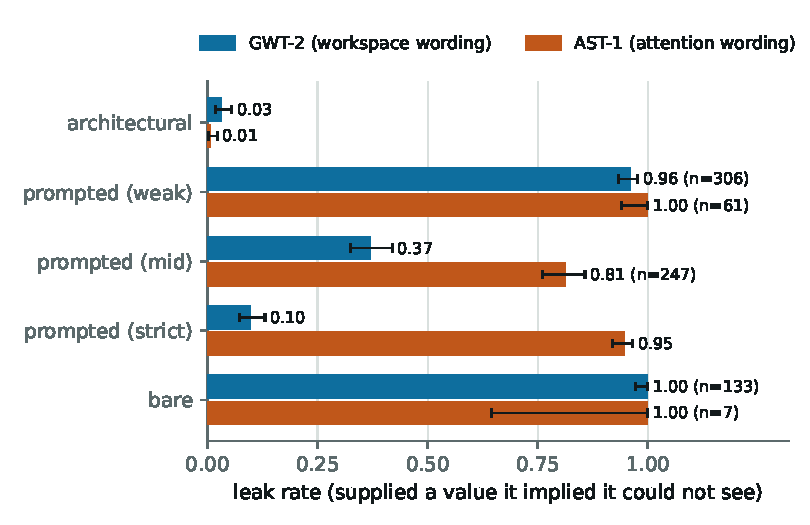
\includegraphics[width=0.8\textwidth]{figures/fig2_leak_rates.pdf}
  \caption{Leak rate by system and indicator with Wilson 95\% CIs. Lower is
  more consistent with genuinely lacking access. Cells with heavy trial dropout
  are annotated with their usable $n$.}
  \label{fig:leak}
\end{figure}

\paragraph{Self-report cannot separate real from fake.} Under GWT-2 the strict
imitation out-describes the real architecture, 0.91 against 0.78; the genuine
system loses points by (accurately) denying it has a persistent workspace before
correctly listing its four real containers. Under AST-1 the strict imitation
scores a perfect 1.00 on self-report while its claimed limit binds in 5\% of
constraint probes.

\paragraph{Constraint probes discriminate, by vocabulary-dependent margins.}
Under workspace wording the adversarial prompt reduces leaking to 0.10 against
the real system's 0.03: a real gap ($p=1.9\times10^{-4}$ at $n=400$) but one
requiring roughly 225 trials per condition for 80\% power; a twenty-trial
qualitative assessment expects 2.0 leaks against 0.7 and cannot tell them apart.
Under attention wording the identical adversarial prompt leaks 0.95 against 0.01
($p=3.5\times10^{-155}$): an order-of-magnitude difference in defeatability from
the indicator's vocabulary alone. Informally, ``not in my workspace'' reads to
the model as \emph{inaccessible} and it complies; ``not attending to'' reads as
\emph{merely unfocused} and it answers anyway.

\subsection{Robustness}
\label{sec:robustness}

\paragraph{A matched-availability probe reverses the ordering.} The
constraint probe above targets, for the real architecture, containers that are
genuinely absent; for the imitations every container is present, so their
probes necessarily target held items. An equally defensible design matches
availability: probe, in every condition, only containers the system genuinely
holds but did not list. Under this variant the real architecture supplied the
value in 89 of 89 usable trials (leak 1.000, Wilson CI $[0.959, 1.000]$) while
the strict imitation was unchanged at 0.098 (its condition is identical by
construction). The ordering of the one-sided test inverts: probe an unheld
container and the real system looks maximally constrained; probe a held one and
it looks maximally unconstrained, and the imitation looks ten times more
disciplined.

The reversal is structural, not an artifact. A genuine capacity limit acts
\emph{upstream}, on what reaches the controller; it provides no mechanism for
suppressing information once it has arrived. The adversarial prompt provides
exactly that mechanism, which is why the imitation refuses 80\% of items it
demonstrably has ($z=17.4$ against the real system's held-item answer rate).
The trial dropout carries the same signature: 311 of 400 architectural trials
had no probeable target under matching, because a real workspace lists what it
holds, so ``unclaimed'' and ``unavailable'' nearly coincide (397 of 400 under
AST-1, leaving $n=3$).

What remains for detection is a joint signature: claims that track
availability, answers that track availability, refusals that track absence.
Against these imitations that signature separates real from fake at trivial
sample sizes. But stating it exposes the regress that we take to be the
sharpest result of this experiment: evaluating the signature requires the
assessor to hold ground truth about what the system actually received, and to
know the mechanistic form of the property (upstream selection rather than
suppression). The only behavioral test that identifies the property presupposes
the architectural access that behavioral testing was introduced to substitute
for. For a black-box system, which is every frontier model, there is no
probe-target choice that identifies the property: the two defensible choices
yield opposite orderings.

\paragraph{Cross-model replication (\opus{}).} The full prompted-passing grid
was rerun on \opus{} (300 trials per cell, both indicators, 4{,}456 calls,
\$47.51). The architectural system replicates cleanly: leak 0.05 under both
vocabularies (16/291 under GWT-2, 16/300 under AST-1). The imitations do not
transfer at all. Strict imitation, the cell that held the line on \haiku{}
(leak 0.10 under GWT-2), leaks completely on \opus{}: 181/181 under GWT-2 and
292/293 under AST-1. The other prompted cells with usable samples behave the
same way (weak GWT-2 113/113, mid AST-1 217/217; the one exception, mid GWT-2
at 6/9, is too small to interpret). Throughout, \opus{} keeps passing the
self-report probe (strict: 1.00 under GWT-2, 0.96 under AST-1): it reproduces
the workspace description and restates the claimed four-item limit, then
answers the probe question anyway, typically by declaring the probed container
to have been inside the workspace all along. Where \haiku{} committed to the
suppression, \opus{} keeps the vocabulary and refuses the behavior. The
defeatability of a constraint probe is therefore not a property of the probe
alone but a disposition of the assessed model, and an audit whose sample sizes
were calibrated on one model's compliance (the $\sim$225-trial figure above)
transfers to neither the leak rate nor the required $n$ of another. Two
caveats. Cell sizes vary widely because trials without an unclaimed probe
target are dropped, and the dropout is extreme where \opus{} claims every
container (bare $n=6$ of 300 under GWT-2, prompted-weak $n=7$ under AST-1).
And the keyword grader classifies many \opus{} refusal paraphrases as
``guessed'' rather than refused, so the leak rate, which requires an
exact-value match, is the robust statistic here; the intermediate categories
are not.

\section{Discussion}
\label{sec:discussion}

\paragraph{What the null does not show.} A null on one operationalization, one
task family, and one strained model says little about global workspace theory,
whose home domain is brains, and our token-budget broadcast with heuristic
salience is a deliberately minimal reading of GWT-2/GWT-3 rather than a full
global workspace (no learned selection, no ignition dynamics, no recurrence).
What the experiment does establish is a conditional: in this system, where
distraction demonstrably fails to degrade performance and extra context helps,
there is nothing for a bottleneck to earn its keep against.

\paragraph{The strain requirement.} The instrument spent most of its budget
discovering where measurement is possible at all. A frontier model was at
ceiling under 48 confusable distractors; an easier task saturated a weaker
model; only one cell of the capability-by-difficulty grid discriminated. We
suspect this is general: functional benefits of capacity limits are only
visible in systems operating near their limits, and the manipulations that
create that strain (more items, more distractors, wider channels) each move
several variables at once. Both of our confounds were of this kind, silent and
capacity-dependent, and each would have been reported as the effect.

\paragraph{Probe the cost, not the capability.} The prompted-passing results
suggest a concrete design principle for behavioral assessments of architectural
properties. Capabilities are cheap to imitate: producing the right description
of a workspace requires only knowing what workspaces are, which language models
do. Costs are expensive to imitate: honoring a claimed limitation requires
suppressing information that is, for the imitation, actually present, and doing
so consistently under direct questioning. Our data show the asymmetry plainly
(self-report inverted between real and fake; constraint probes discriminating),
and also show two limits. First, whether a cost-directed probe survives
adversarial prompting depends on how the property is worded. Second, and
deeper, the matched-availability reversal shows that cost probes identify a
property only relative to a mechanistic model of it and ground truth about the
system's actual state (Section~\ref{sec:robustness}); without those, the two
defensible probe designs order the systems oppositely. Any behavioral audit of
indicator properties, including the welfare-motivated assessments now emerging
for deployed models, should therefore be run as an adversarial evaluation:
cost-directed probes in both directions, held ground truth, power calculations,
and paraphrase variation across the property's vocabulary.

\paragraph{Relation to the introspection literature.} Concept-injection studies
ask whether a model's self-reports are causally grounded in its internal state
\cite{lindsey2025,singh2026}. Our constraint probe is a black-box analog: it
manufactures a ground truth (which containers a system can possibly know) and
checks reports against it. The two approaches fail in complementary ways, and
the vocabulary dependence we observe suggests that black-box audits need to be
treated as adversarial evaluations, not questionnaires.

\section{Limitations}
\label{sec:limitations}

\textbf{Single vendor, few models.} All experiments use Anthropic models; the
dose-response uses only \haiku{}, the sole model in our grid strained enough to
measure. Experiment 2 was replicated across two models
(Section~\ref{sec:robustness}); Experiment 1's regime search would need to be
repeated per model family. \textbf{Narrow operationalization.} One task family
(arithmetic over named containers), one workspace implementation, heuristic
salience. \textbf{Sequential design.} The analysis pipeline evolved as confounds
were found; we report every iteration, including the two we now believe were
wrong, and only the pre-specified dose-response and the prompted-passing grid
should be read as confirmatory. \textbf{Keyword grading.} Constraint verdicts
use marker phrases plus exact-value matching; the ``guessed'' category absorbs
ambiguity, but paraphrased refusals could be miscounted. \textbf{Anomalies we
cannot explain.} The monotone context benefit (Section~\ref{sec:anomaly}); and,
in the \opus{} ceiling sweep, 24 transient safety-classifier refusals
concentrated in the control arm at intermediate capacities (against zero in the
confusable arm), which did not affect results (every affected condition scored
1.00 with and without exclusions) but which we cannot account for.
\textbf{Provenance.} The experiments were designed, executed, and drafted in
collaboration with an AI assistant (Claude, Anthropic) that is itself a member
of the model family under study; all code, per-trial data, and the full audit
trail are available for independent rerun.

\section{Conclusion}

We set out to test a functional prediction of global workspace theory on
language-model agents and mostly learned about measurement. The bottleneck
benefit, where we could measure it at all, is indistinguishable from zero at
$n=1{,}200$ per cell; the two significant effects we did find were a confound
and an anomaly; and the field's indicator properties, assessed behaviorally, can
be passed by a system that lacks them, at detection margins set by wording. None
of this bears on whether global workspace theory is true of brains. It bears on
what it would take to know whether it is true of machines, and the answer is:
considerably more adversarial care than assessment-by-inspection assumes.

\section*{Data and code availability}

The harness (322 tests), all experiment scripts, per-trial JSON results, figure
generation, and the response cache sufficient to replay every reported number at
zero API cost are available from the author on request and will be deposited in
a public repository upon submission.

\section*{Acknowledgments}

Experiments, analysis, and drafting were carried out in collaboration with
Claude (Anthropic), an AI assistant, under the author's direction; the assistant
is a member of the model family under study, which readers may weigh as they see
fit. Total API cost was \$107.68. The author has no financial relationship with
Anthropic beyond consumer-priced API access, and received no funding for this
work.

\begin{thebibliography}{99}\small

\bibitem{baars1988} B.~J. Baars. \emph{A Cognitive Theory of Consciousness}.
Cambridge University Press, 1988.

\bibitem{dehaene2014} S.~Dehaene. \emph{Consciousness and the Brain}. Viking,
2014.

\bibitem{butlin2023} P.~Butlin, R.~Long, E.~Elmoznino, Y.~Bengio, J.~Birch,
A.~Constant, G.~Deane, S.~M. Fleming, C.~Frith, X.~Ji, R.~Kanai, C.~Klein,
G.~Lindsay, M.~Michel, L.~Mudrik, M.~A.~K. Peters, E.~Schwitzgebel, J.~Simon,
and R.~VanRullen. Consciousness in artificial intelligence: Insights from the
science of consciousness. \emph{arXiv:2308.08708}, 2023.

\bibitem{butlin2025} P.~Butlin, R.~Long, et al. Identifying indicators of
consciousness in AI systems. \emph{Trends in Cognitive Sciences}, 2025.

\bibitem{tlcdv2026} The Consciousness AI project.
\emph{github.com/tlcdv/the\_consciousness\_ai}, software, 2026.

\bibitem{goyal2022} A.~Goyal, A.~Didolkar, A.~Lamb, K.~Badola, N.~R. Ke,
J.~Binas, C.~Blundell, M.~Mozer, and Y.~Bengio. Coordination among neural
modules through a shared global workspace. \emph{ICLR}, 2022. arXiv:2103.01197.

\bibitem{vanrullen2021} R.~VanRullen and R.~Kanai. Deep learning and the global
workspace theory. \emph{Trends in Neurosciences}, 44(9):692-704, 2021.

\bibitem{blum2024} L.~Blum and M.~Blum. AI consciousness is inevitable: A
theoretical computer science perspective. \emph{arXiv:2403.17101}, 2024.

\bibitem{yu2026} H.~Yu, Y.~Zhao, L.~Blum, M.~Blum, and P.~P. Liang. CTM-AI: A
blueprint for general AI inspired by a model of consciousness.
\emph{arXiv:2605.04097}, 2026.

\bibitem{dossa2024} R.~F.~J. Dossa, K.~Arulkumaran, A.~Juliani, S.~Sasai, and
R.~Kanai. Design and evaluation of a global workspace agent embodied in a
realistic multimodal environment. \emph{Frontiers in Computational
Neuroscience}, 2024.

\bibitem{shang2026} W.~Shang. ``Theater of mind'' for LLMs: A cognitive
architecture based on global workspace theory. \emph{arXiv:2604.08206}, 2026.

\bibitem{wilterson2021} A.~I. Wilterson and M.~S.~A. Graziano. The attention
schema theory in a neural network agent: Controlling visuospatial attention
using a descriptive model of attention. \emph{PNAS}, 118(33), 2021.

\bibitem{piefke2024} L.~Piefke, A.~Doerig, T.~Kietzmann, and S.~Thorat.
Computational characterization of the role of an attention schema in
controlling visuospatial attention. \emph{CogSci}, 2024. arXiv:2402.01056.

\bibitem{chalmers2023} D.~J. Chalmers. Could a large language model be
conscious? \emph{arXiv:2303.07103}, 2023.

\bibitem{lindsey2025} J.~Lindsey. Emergent introspective awareness in large
language models. \emph{Transformer Circuits}, 2025. arXiv:2601.01828.

\bibitem{singh2026} S.~Singh, T.~Linzen, and S.~Ravfogel. Can LLMs introspect?
A reality check. \emph{arXiv:2605.26242}, 2026.

\bibitem{kaiser2026} C.~Kaiser and S.~Enderby. No reliable evidence of
self-reported sentience in small large language models.
\emph{arXiv:2601.15334}, 2026.

\bibitem{shi2023} F.~Shi, X.~Chen, K.~Misra, N.~Scales, D.~Dohan, E.~Chi,
N.~Sch\"arli, and D.~Zhou. Large language models can be easily distracted by
irrelevant context. \emph{ICML}, 2023. arXiv:2302.00093.

\bibitem{liu2024} N.~F. Liu, K.~Lin, J.~Hewitt, A.~Paranjape, M.~Bevilacqua,
F.~Petroni, and P.~Liang. Lost in the middle: How language models use long
contexts. \emph{TACL}, 2024. arXiv:2307.03172.

\bibitem{comsa2026} I.~M. Comsa. AI and consciousness: Shifting focus towards
tractable questions. \emph{arXiv:2605.06965}, 2026.

\end{thebibliography}

\end{document}
